\chapter[phd_state_of_the_art]{State of the Art}
[
    This chapter reviews the placeholder literature, and positions the contribution of \nameref{phd_contribution} with respect to it.
]

    \section[phd_sota_early]{Early Approaches}

        Lorem ipsum dolor sit amet, consectetur adipiscing elit~\cite{ipsum1998foundational}.
        Sed do eiusmod tempor incididunt ut labore et dolore magna aliqua, as summarized in the textbook of \cite{tempor2009textbook}.

        \begin{boxenv}[phd_definition]{Definition}[Placeholder representation]
            A \emph{placeholder representation} of an observation $\bm{x}$ is any vector $\bm{z} = g(\bm{x})$ such that $\bm{z}$ carries no more information than $\bm{x}$.
        \end{boxenv}

    \section[phd_sota_modern]{Modern Approaches}

        Ut enim ad minim veniam, quis nostrud exercitation ullamco laboris nisi ut aliquip ex ea commodo consequat~\cite{amet2017seminal}.
        \acro{cnn_plural} are now trained on a single \acro{gpu}, which was not the case for the earlier approaches of \nameref{phd_sota_early}.
        \nameref{phd_sota_figure} summarizes the pipeline they all share.

        \begin{figure}[phd_sota_figure]{An overview of the placeholder pipeline shared by modern approaches. The same figure is reused in \nameref{phd_contribution}, which is perfectly fine as long as the labels differ.}
            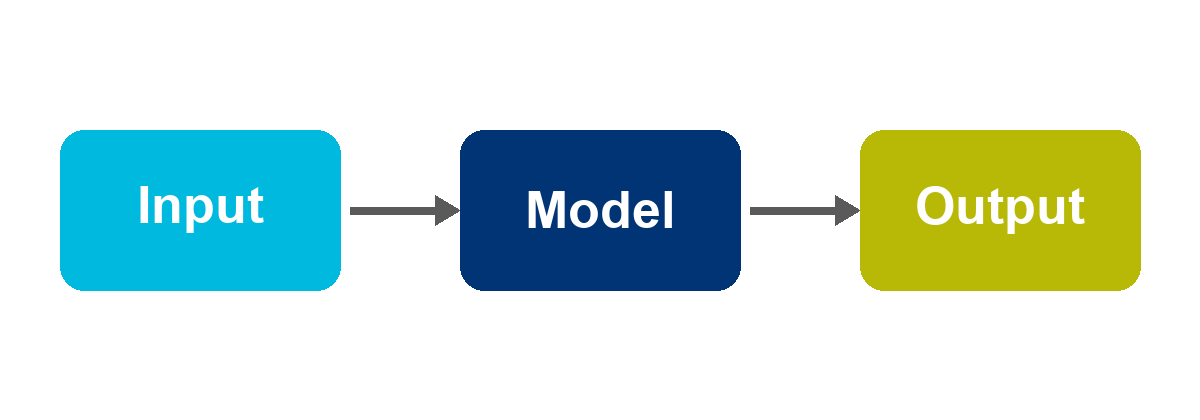
\includegraphics[width=0.9\linewidth]{manuscript/figures/example_diagram.png}
        \end{figure}

    \section[phd_sota_summary]{Summary}

        \nameref{phd_sota_table} compares the approaches discussed above.
        None of them addresses \nameref{phd_problem_box} directly, which motivates the contribution of \nameref{phd_contribution}.

        \begin{table}[phd_sota_table]{A comparison of placeholder approaches. Checkmarks are placeholders too.}
            \begin{tabular}{lccc}
                \hline
                \textbf{Approach} & \textbf{Placeholder} & \textbf{Scalable} & \textbf{Interpretable} \\
                \hline
                \cite{ipsum1998foundational} & \faCheck & \faTimes & \faCheck \\
                \cite{tempor2009textbook} & \faCheck & \faTimes & \faTimes \\
                \cite{amet2017seminal} & \faCheck & \faCheck & \faTimes \\
                \textbf{Ours} & \faCheck & \faCheck & \faCheck \\
                \hline
            \end{tabular}
        \end{table}
